\documentclass{beamer}

\usepackage[utf8]{inputenc}
\usepackage{default}
\usepackage{soul}
\makeatletter
\newcommand\SoulColor{%
  \let\set@color\beamerorig@set@color
  \let\reset@color\beamerorig@reset@color}
\makeatother

\newcommand*\MyPitem{%
  \item[\color{green}\scalebox{0.9}{\textbullet}]}
\newcommand*\MyCitem{%
  \item[\color{red}\scalebox{0.9}{\textbullet}]}

\begin{document}

\let\tempone\itemize
\let\temptwo\enditemize
\renewenvironment{itemize}{\tempone\addtolength{\itemsep}{0.5\baselineskip}}{\temptwo}

\begin{frame}{Distant supervision for Numerical Relation Extraction}{Knowledge Base}
 \begin{itemize}
  \item Derived from \url{data.worldbank.org}, 4371979 numerical facts about 249 countries, 1281 attributes 

\begin{tabular}{|l|l|l|}
\hline
/m/04g5k&3126000130&EG.ELC.PROD.KH\\
/m/02k8k&1969.179&EN.ATM.CO2E.KT\\
/m/06nnj&332315&SP.POP.TOTL\\
/m/019rg5&55.020073&SP.DYN.LE00.IN\\
/m/05sb1&19974.148&EN.ATM.CO2E.KT\\
/m/05v8c&10000000000&EG.ELC.PROD.KH\\
/m/03spz&7639000100&EG.ELC.PROD.KH\\
/m/06vbd&44249.688&EN.ATM.CO2E.KT\\
/m/0d060g&51.3&IT.NET.USER.P2\\
/m/05qkp&62.298927&SP.DYN.LE00.IN\\
\hline
\end{tabular}


\end{itemize}

\end{frame}

\begin{frame}{Selected Relations}
 \begin{center}
\begin{tabular}{|l|l|}
\hline
Relation Name & Relation Code \\
\hline
Land area (sq. km)&AG.LND.TOTL.K2\\
Foreign direct investment, net (current US\$)&BN.KLT.DINV.CD\\
Goods exports (current US\$)&BX.GSR.MRCH.CD\\
Electricity production (kWh)&EG.ELC.PROD.KH\\
CO2 emissions (kt)&EN.ATM.CO2E.KT\\
Pump price for diesel fuel (US\$ per liter)&EP.PMP.DESL.CD\\
Inflation, consumer prices (annual \%)&FP.CPI.TOTL.ZG\\
Internet users (per 100 people)&IT.NET.USER.P2\\
GDP (current US\$)&NY.GDP.MKTP.CD\\
Life expectancy at birth, total (years)&SP.DYN.LE00.IN\\
Population (Total)&SP.POP.TOTL\\
\hline
\end{tabular}
\end{center}

\end{frame}

\begin{frame}{Corpus}
\begin{itemize}
 \item Subset of the tac corpus
 \item 268, 036 Documents, X sentences having a country and a number 
 \item List of countries augmented manually by adding all possible synonyms (Dutch, Netherlands) and inflections (Ireland, Irish)
\end{itemize}

 
\end{frame}

\begin{frame}{Distant supervision process for numerical relation extraction}
 \begin{itemize}
  \item Extract a country and number from a sentence, go to kb and check if there is a match.
  \item Can be creative during matching:
  \begin{itemize}
   \item Distance based matching
   \item Time based matching
  \end{itemize}
 \end{itemize}
\end{frame}

\begin{frame}{False Positives}{Numbers are weak entities}
\begin{itemize}
 \item Vanilla numerical relation matching is bound to attract humoungous amounts of false positives;
 \item Stems from the fact that numbers don't have an identity of their own.
 \item Consider {\SoulColor\hl{India}} and {\SoulColor\hl{Mumbai}} Vs. {\SoulColor\hl{India}} and {\SoulColor\hl{19}}
 \item {\SoulColor\hl{Mumbai}} is a strong entity, {\SoulColor\hl{19}} is a \textbf{weak} entity.
 \end{itemize}
\end{frame}


 \begin{frame}{False Positives}{Numbers are weak entities}
 \begin{itemize}  
 \item Compare the number of sentences in which {\SoulColor\hl{India}} and {\SoulColor\hl{Mumbai}} appear together, vs the number of sentences
  in which {\SoulColor\hl{India}} and {\SoulColor\hl{19}} appear together.
 \item Just {\SoulColor\hl{19}} can be appear with India in several contexts:
 \begin{itemize}
 \item Internet user \%
 \item Billion dollars invested by a company
 \item \% of people below the poverty line
 \item date (if we are not careful)
 \item number of medals won by Indian athletes...
\end{itemize}

 \item Can we expect the situation to be even worse for certain types of numbers?
\end{itemize}
\end{frame}

\begin{frame}{One Thousand Words}
 \begin{center}
 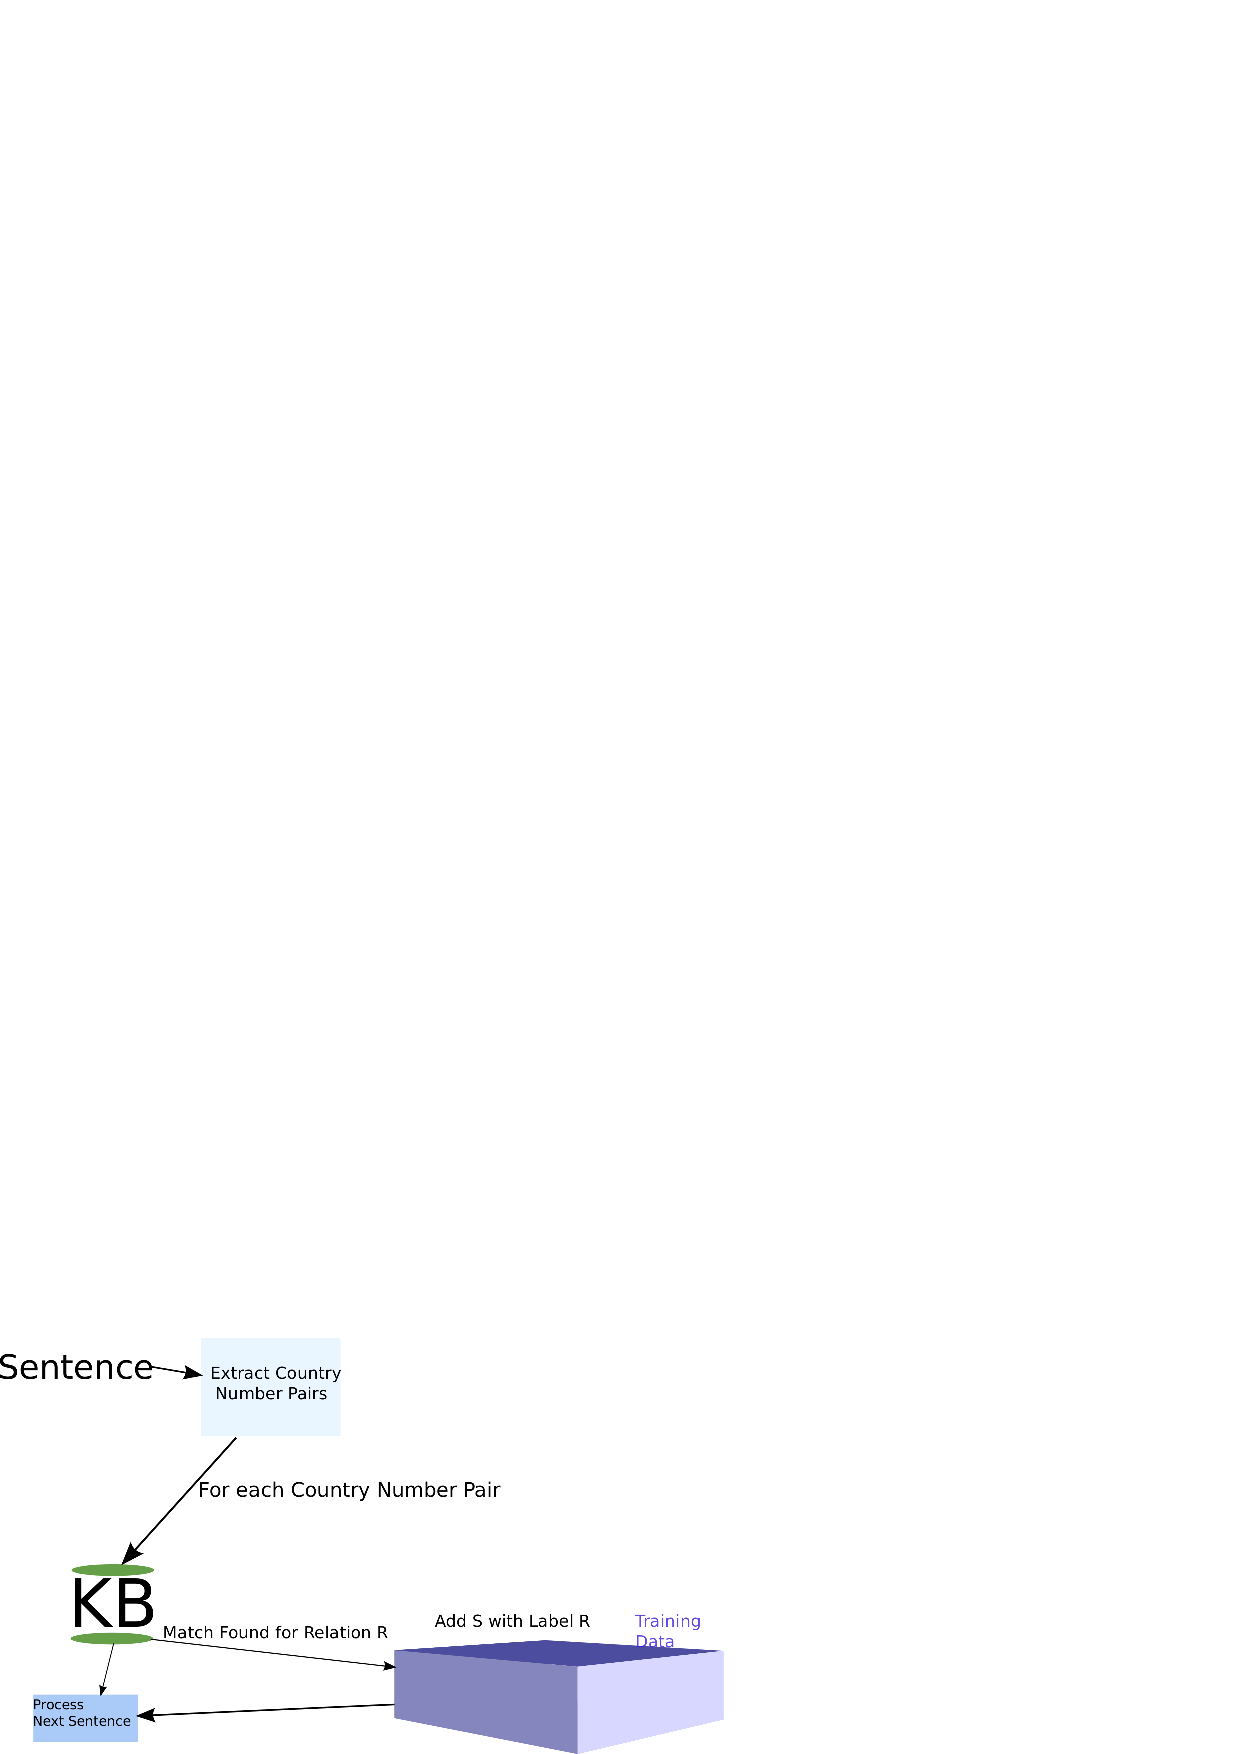
\includegraphics{./imgs/simple.pdf}
 % simple.pdf: 363x272 pixel, 72dpi, 12.81x9.60 cm, bb=0 0 363 272
\end{center}

\end{frame}


\end{document}
